\documentclass[tikz,border=6pt]{standalone}
% Shared visual language for the book's standalone vector figures.
% Keep this file compatible with the TeX Live version used by LyX.
\usepackage{amsmath,amssymb}
\usepackage{array,booktabs}
\usepackage{pgfplots}
\usepackage{pgfplotstable}
\usetikzlibrary{arrows.meta,calc,positioning}
\pgfplotsset{compat=1.17}

\definecolor{BookBlue}{HTML}{0072B2}
\definecolor{BookOrange}{HTML}{D55E00}
\definecolor{BookGreen}{HTML}{009E73}
\definecolor{BookGray}{HTML}{666666}
\definecolor{BookLightGray}{HTML}{D9D9D9}

\pgfplotsset{
  book axis/.style={
    axis line style={black!75,line width=0.55pt},
    tick style={black!75,line width=0.45pt},
    tick label style={font=\small},
    label style={font=\small},
    legend style={
      font=\small,
      draw=none,
      fill=none,
      cells={anchor=west},
    },
    grid style={BookLightGray,line width=0.35pt},
    major grid style={BookLightGray,line width=0.35pt},
  },
}

\usepgfplotslibrary{groupplots}
\begin{document}
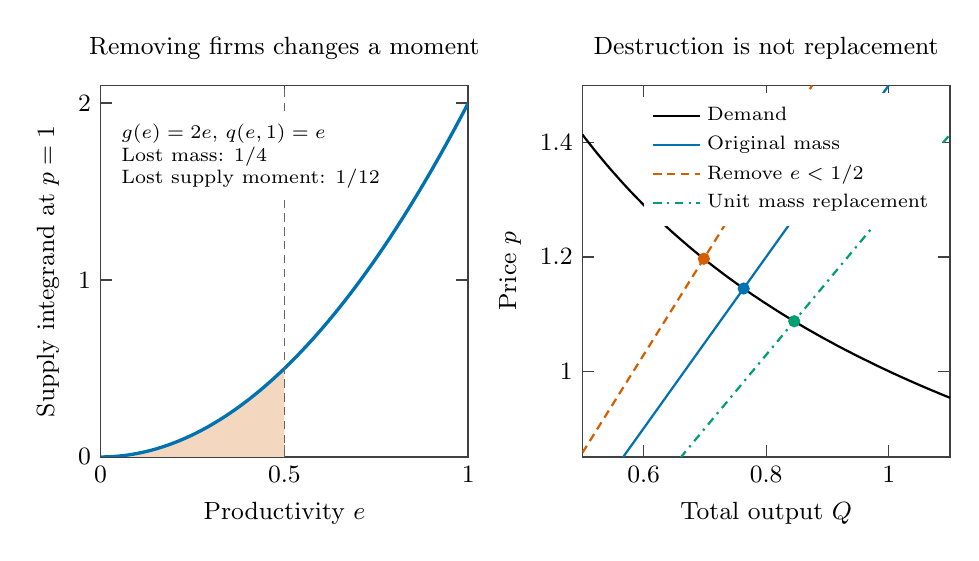
\begin{tikzpicture}
\begin{groupplot}[group style={group size=2 by 1,horizontal sep=1.45cm},
 book axis,width=6.25cm,height=6.3cm,title style={font=\small,align=center}]
 \nextgroupplot[xmin=0,xmax=1,ymin=0,ymax=2.1,xlabel={Productivity $e$},
 ylabel={Supply integrand at $p=1$},xtick={0,.5,1},ytick={0,1,2},
 title={Removing firms changes a moment}]
 \addplot[draw=none,fill=BookOrange!25,domain=0:.5,samples=60] {2*x^2}\closedcycle;
 \addplot[BookBlue,very thick,domain=0:1,samples=100]{2*x^2};
 \draw[densely dashed,BookGray] (axis cs:.5,0)--(axis cs:.5,2.1);
 \node[anchor=west,font=\scriptsize,fill=white,align=left] at(axis cs:.03,1.7)
 {$g(e)=2e$, $q(e,1)=e$\\Lost mass: $1/4$\\Lost supply moment: $1/12$};
 \nextgroupplot[xmin=.5,xmax=1.1,ymin=.85,ymax=1.5,xlabel={Total output $Q$},
 ylabel={Price $p$},title={Destruction is not replacement},
 legend style={at={(.98,.98)},anchor=north east,font=\scriptsize,
   fill=white,fill opacity=1,text opacity=1,inner sep=3pt}]
 \addplot[black,thick,domain=.5:1.1,samples=100]{1/sqrt(x)};
 \addlegendentry{Demand}
 \addplot[BookBlue,thick,domain=.5:1.0]{1.5*x};
 \addlegendentry{Original mass}
 \addplot[BookOrange,thick,densely dashed,domain=.5:.875]{12*x/7};
 \addlegendentry{Remove $e<1/2$}
 \addplot[BookGreen,thick,dashdotted,domain=.66:1.1]{9*x/7};
 \addlegendentry{Unit mass replacement}
 \addplot[only marks,mark=*,BookBlue] coordinates{({(2/3)^(2/3)},{(3/2)^(1/3)})};
 \addplot[only marks,mark=*,BookOrange] coordinates{({(7/12)^(2/3)},{(12/7)^(1/3)})};
 \addplot[only marks,mark=*,BookGreen] coordinates{({(7/9)^(2/3)},{(9/7)^(1/3)})};
\end{groupplot}
\end{tikzpicture}
\end{document}
